% FileName: ./HeatSink.tex
% Generated by: AcuReport
% Date: Thu Dec 23 01:48:49 Iran Standard Time 2010
\documentclass[letterpaper,12pt]{article}
\usepackage{graphicx}
\usepackage{hyperref}
\usepackage{cooltooltips}
\usepackage[3D]{movie15}
\addtolength{\oddsidemargin}{-.875in}
\addtolength{\evensidemargin}{-.875in}
\addtolength{\textwidth}{1.75in}
\addtolength{\topmargin}{-.875in}
\addtolength{\textheight}{1.75in}
\begin{document}
\hypersetup{pdfborder={0 0 0} }
\begin{center}
\includegraphics[scale=0.508026823816]{./Figures/CFDCalcLogo.png}
\end{center}
\vspace*{2.00mm}\hspace*{\fill}\\
\begin{center}
\Large{ \textsc{ Heat Sink Calculator\\Version 1.0 }}\\
\end{center}
\vspace*{1.00mm}\hspace*{\fill}\\
\begin{center}
Heat Sink Model\\Steady Rans Simulation\\
\end{center}
\begin{center}
Thu Dec 23 13:49:05 2010\\
\end{center}
\vspace*{1.00mm}\hspace*{\fill}\\
\vfill
\begin{center}
\emph{Product of CFDCalc}\\
\end{center}
\begin{center}
http://www.cfdcalc.com\\
\end{center}
\vfill
\newpage
\clearpage
\tableofcontents
\vfill
\newpage
\clearpage
\section{Problem Description}

Heatsink design is one of the most important part of electronic design.
This report presents parametric heatsink solutions based 
on AcuSolve software suite for advanced CFD simulations. A series of 
test cases can be computed with multiple airflow simulations, at 
variour flow rates. The simulations can help you choose the best 
heatsink solution, whether hermal performance or a combination of 
factors such as cost, weight, or influence on the overall system 
pressure drop.
\\
\section{Model Setup}

The geometry CAD files are created using 
\\
\subsection{CAD Properties}

In this section, you can see the CAD
properties and views as well as an interactive view of
the heat sink problem.
\\
The following are the user input data for heat sink problem:\\
\begin{flushleft}
\begin{tabular}{ l l }
Tunnel Dimensions: & 304.10 x 152.10 x 152.10 $mm^3$ \\
Board Dimensions: & 76.21 x 114.31 x 1.61 $mm^3$ \\
Chip Dimensions: & 12.10 x 12.10 x 1.10 $mm^3$ \\
Heat Sink Type: & Cross Cut \\
Heat Sink Dimensions: & 25.41 x 25.41 x 10.10 $mm^3$ \\
Heat Sink Base Height: & 2.10 mm \\
Fin X-Width: & 2.10 mm \\
Fin X-Gap: & 2.10 mm \\
Number of X-Fins: & 6 \\
Side X-Gap: & 1.16 mm \\
Fin Y-Width: & 2.10 mm \\
Fin Y-Gap: & 2.10 mm \\
Number of Y-Fins & 6 \\
Side Y-Gap: & 1.16 mm \\
Mesh Density: & Coarse \\
Package Theta JC: & 3.10  \\
Package Theta JB: & 3.10  \\
Fluid Material Model: & Air  \\
Heat Sink Material model: & Copper  \\
Board Layer Parameters: & [  1.40000000e-03   9.90000000e+01]  \\
Solution Cases, Air Speed: & [ 1.1  2.1  1.1] m/sec \\
Solution Cases, Temperature: & [ 293.25  293.25  313.25] K \\
Solution Cases, Chip Power: & [ 10.1  10.1  10.1] W \\
\end{tabular}
\end{flushleft}
\vfill
\newpage
\clearpage
\subsubsection{CAD View}
\begin{figure}[!h!tbp]
\begin{center}
\includegraphics[scale=0.232399179768]{./Figures/IsometricView.png}
\caption{\label{fig:isometric}Isometric View}
\end{center}
\end{figure}
\begin{figure}[!h!tbp]
\begin{center}
\includegraphics[scale=0.232399179768]{./Figures/TopView.png}
\caption{\label{fig:top}Top View}
\end{center}
\end{figure}
\begin{figure}[!h!tbp]
\begin{center}
\includegraphics[scale=0.232399179768]{./Figures/FrontView.png}
\caption{\label{fig:front}Front View}
\end{center}
\end{figure}
\begin{figure}[!h!tbp]
\begin{center}
\includegraphics[scale=0.232399179768]{./Figures/SideView.png}
\caption{\label{fig:side}Side View}
\end{center}
\end{figure}
\vfill
\newpage
\clearpage
\subsubsection{Interactive View}
Click on the following control to activate it.
You may use mouse buttons or toolbar controls to manipulate
the interactive 3D model of the heat sink problem.\\
Please review the footnote comment\footnotemark
to find out how to use the following control.

\footnotetext{To start, click on the control to activate it.
\begin{itemize}
\item{\textbf{If you cannot see the model properly,
click on the \emph{Model Tree} from the \emph{Navigation Panels},
then right click on the root node and choose either
\emph{Zoom to Part} or \emph{Fit Visible}.}}

\item{To enable double-sided rendering, go to
\emph{Edit} $\rightarrow$ \emph{Preferences} $\rightarrow$ \emph{3D}
and check the \emph{Enable double-sided rendering} option.}

\item{You can toggle between the perspective and orthographic views
by clicking in the \emph{Cube} icon on the control toolbar.}

\item{You may use mouse buttons or toolbar controls to manipulate
the interactive 3D model.}

\end{itemize} }

\begin{center}
\includemovie[
	poster,
	toolbar, %same as `controls
	3Daac=40.000000,
	3Droll=0.000000,
	3Dc2c=0.000000 0.000000 1.000000,
	3Droo=0.304200,
	3Dcoo=0.000000 0.000000 0.000000,
	3Dlights=CAD,
]{\linewidth}{0.67\linewidth}{./Figures/HeatSink.u3d}
\end{center}
\subsection{Mesh Generation}

The quality of grid in general plays an important role on the 
flow and thermal physics for a CFD solver. Once the CAD model of the
heatsink had been created, we discretize the geometry to form a grid that 
is reasonable to capture the dominant flow features. In particular, 
we need to pay attention in the meshing near the wall of heatsink and the
optimized volumetric mesh distribution.
\\
\vfill
\newpage
\clearpage
\section{Results}


Estimating how much the processor case temperature will rise given an increase in power to determining how to manage the additional heat.


We will consider different scenarios....

The cases results of temperature is given in Table \ref{tab:cases1}.
\\
\begin{table}[!h!tbp]
\begin{center}
\begin{tabular}{| l | p{1.5cm} | p{1cm} | p{1cm} | p{2cm} | p{2cm} | p{1.25cm} | p{1.25cm} | p{1.25cm} | p{1.25cm} | }
\hline
Case & A. Speed (m/sec) & A. Temp. (oC) & C. Power (W) & C./S. Heat Flux (W) & C./B. Heat Flux (W) & C./S. Temp. (oC) & C./B. Temp. (oC) & S. Temp. (oC) & J. Temp. (oC) \\
\hline
1 & 1.10 & 293.25 & 10.10 & 4.74 & 0.31 & 94.47 & 123.49 & 44.06 & 109.15 \\
\hline
2 & 2.10 & 293.25 & 10.10 & 4.74 & 0.31 & 74.54 & 104.00 & 24.08 & 89.24 \\
\hline
3 & 1.10 & 313.25 & 10.10 & 4.72 & 0.33 & 51.77 & 79.42 & 22.19 & 66.40 \\
\hline
\end{tabular}
\caption{\label{tab:cases1}
Cases Results of Temperature}
\end{center}
\end{table}
\begin{itemize}
\item{\emph{The Legend of Table \ref{tab:cases1}:\\}}
A. : Air\\C. : Chip\\S. : Sink\\B. : Board\\J. : Junction\\Temp. : Temperature
\end{itemize}
\vfill
\newpage
\clearpage
\begin{equation}
\theta_{sa} = ( sinkTemp - airTemp ) / chipSinkHeat
\end{equation}
The cases results of $\theta$ is given in Table \ref{tab:cases2}.\\
\begin{table}[!h!tbp]
\begin{center}
\begin{tabular}{| l | p{1.5cm} | p{1cm} | p{1cm} | p{1.5cm} | p{1.5cm} | p{1.5cm} | p{1.5cm} | p{1.5cm} | p{1.5cm} | }
\hline
Case & A. Speed (m/sec) & A. Temp. (oC) & C. Power (W) & $\theta_{JC}$ (oC/W) & $\theta_{JB}$ (oC/W) & $\theta_{CS}$ (oC/W) & $\theta_{SA}$ (oC/W) & $\theta_{CA}$ (oC/W) & $\theta_{JA}$ (oC/W) \\
\hline
1 & 1.10 & 293.25 & 10.10 & 3.10 & 3.10 & 10.64 & -52.62 & -41.97 & -18.23 \\
\hline
2 & 2.10 & 293.25 & 10.10 & 3.10 & 3.10 & 10.64 & -56.76 & -46.12 & -20.20 \\
\hline
3 & 1.10 & 313.25 & 10.10 & 3.10 & 3.10 & 6.27 & -61.67 & -55.41 & -24.44 \\
\hline
\end{tabular}
\caption{\label{tab:cases2}
Cases Results of $\theta$}
\end{center}
\end{table}
\begin{itemize}
\item{\emph{The Legend of Table \ref{tab:cases2}:\\}}
A. : Air\\C. : Chip\\Temp. : Temperature
\end{itemize}
\vfill
\newpage
\clearpage
The "Temperature" vs. "Case Number" curve is given in Figure \ref{fig:tempcase}.



The graph shows the slopes for change in temperature over the range ...for ...nearly linear and parallel to each other...
\\
\begin{figure}[!h!tbp]
\begin{center}
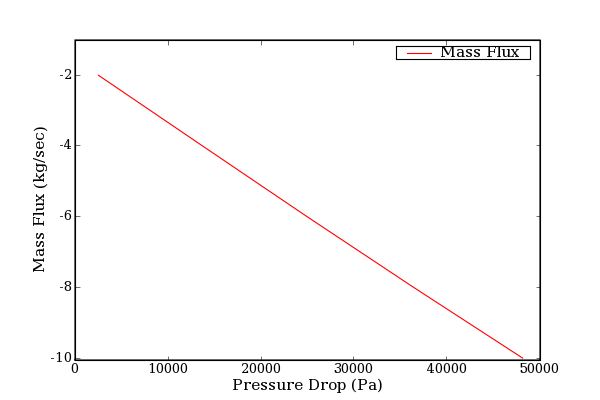
\includegraphics[scale=0.328092959672]{./Figures/plot_1.png}
\caption{\label{fig:tempcase}Temperatures}
\end{center}
\end{figure}
\vfill
\newpage
\clearpage
The "Thermal Resistance" vs. "Case Number" curve is given in Figure \ref{fig:trcase}.\\
\begin{figure}[!h!tbp]
\begin{center}
\includegraphics[scale=0.328092959672]{./Figures/plot_2.png}
\caption{\label{fig:trcase}Thermal Resistances}
\end{center}
\end{figure}
\vfill
\newpage
\clearpage
\subsection{Case 1 Results}
The results of case 1 are given in Figure \ref{fig:case 1}.\\
\begin{itemize}
\item{\emph{Air Speed: 1.10 m/sec}}

\item{\emph{Air Temperature: 293.25 oC}}

\item{\emph{Chip Power: 10.10 W}}

\item{\emph{Junction Temperature: 109.15 oC}}

\end{itemize}
\begin{figure}[!h!tbp]
\begin{center}
\begin{tabular}{ c c }
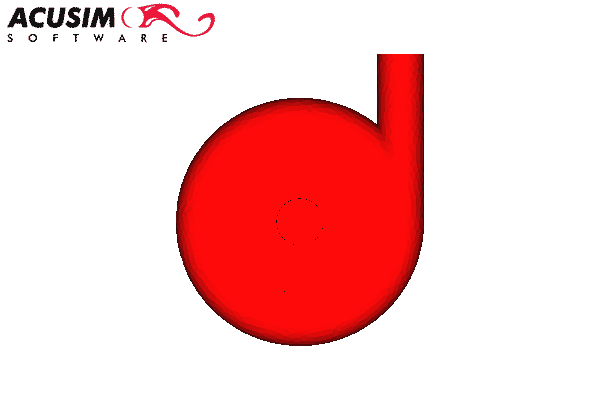
\includegraphics[scale=0.15037593985]{./Figures/Image_0.png}
 & 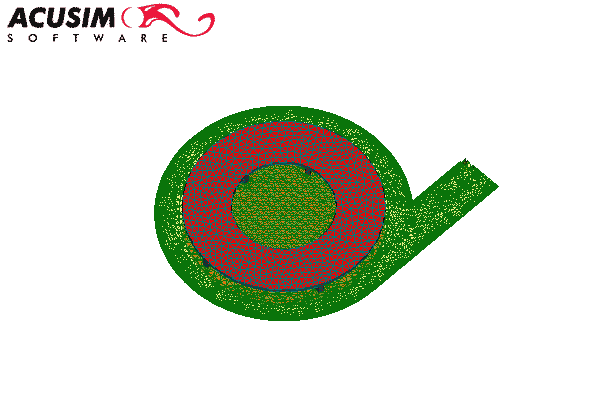
\includegraphics[scale=0.15037593985]{./Figures/Image_1.png}
 \\ Case 1. Surface Temperature & Case 1. Temperature on Cut Plane \\
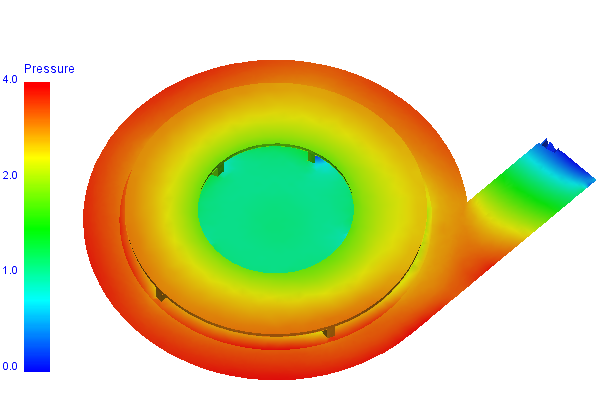
\includegraphics[scale=0.15037593985]{./Figures/Image_2.png}
 &  \\ Case 1. Pressure on Cut Plane &  \\
\end{tabular}
\caption{\label{fig:case 1}
Case 1}
\end{center}
\end{figure}
\vfill
\newpage
\clearpage
\subsection{Case 2 Results}
The results of case 2 are given in Figure \ref{fig:case 2}.\\
\begin{itemize}
\item{\emph{Air Speed: 2.10 m/sec}}

\item{\emph{Air Temperature: 293.25 oC}}

\item{\emph{Chip Power: 10.10 W}}

\item{\emph{Junction Temperature: 89.24 oC}}

\end{itemize}
\begin{figure}[!h!tbp]
\begin{center}
\begin{tabular}{ c c }
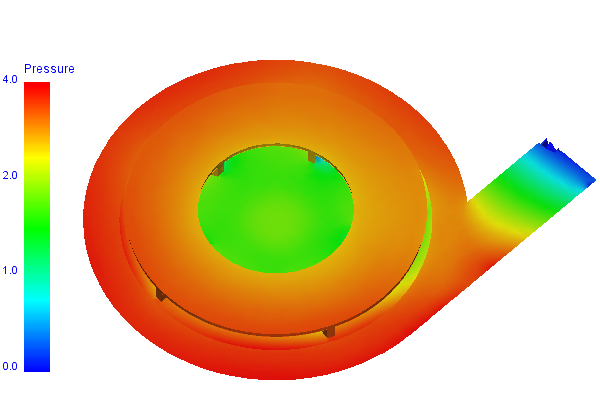
\includegraphics[scale=0.15037593985]{./Figures/Image_3.png}
 & 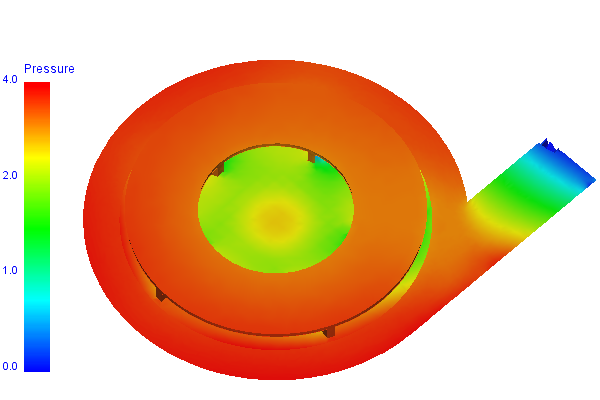
\includegraphics[scale=0.15037593985]{./Figures/Image_4.png}
 \\ Case 2. Surface Temperature & Case 2. Temperature on Cut Plane \\
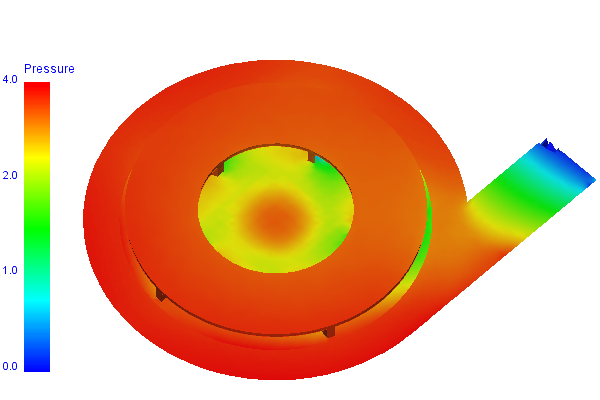
\includegraphics[scale=0.15037593985]{./Figures/Image_5.png}
 &  \\ Case 2. Pressure on Cut Plane &  \\
\end{tabular}
\caption{\label{fig:case 2}
Case 2}
\end{center}
\end{figure}
\vfill
\newpage
\clearpage
\subsection{Case 3 Results}
The results of case 3 are given in Figure \ref{fig:case 3}.\\
\begin{itemize}
\item{\emph{Air Speed: 1.10 m/sec}}

\item{\emph{Air Temperature: 313.25 oC}}

\item{\emph{Chip Power: 10.10 W}}

\item{\emph{Junction Temperature: 66.40 oC}}

\end{itemize}
\begin{figure}[!h!tbp]
\begin{center}
\begin{tabular}{ c c }
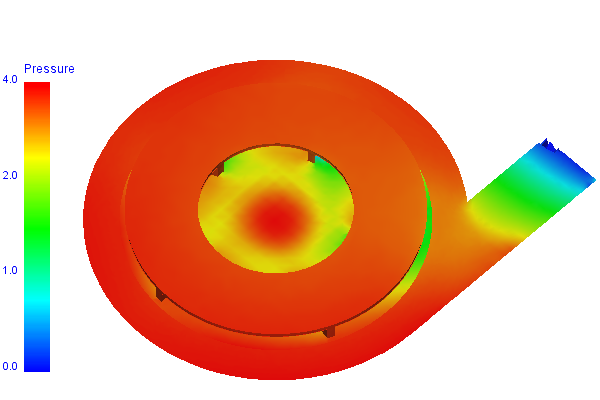
\includegraphics[scale=0.15037593985]{./Figures/Image_6.png}
 & 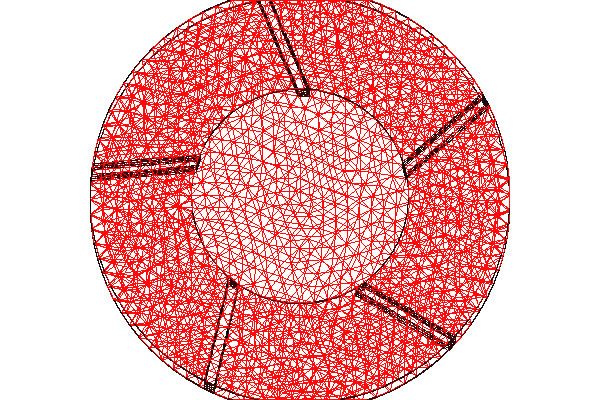
\includegraphics[scale=0.15037593985]{./Figures/Image_7.png}
 \\ Case 3. Surface Temperature & Case 3. Temperature on Cut Plane \\
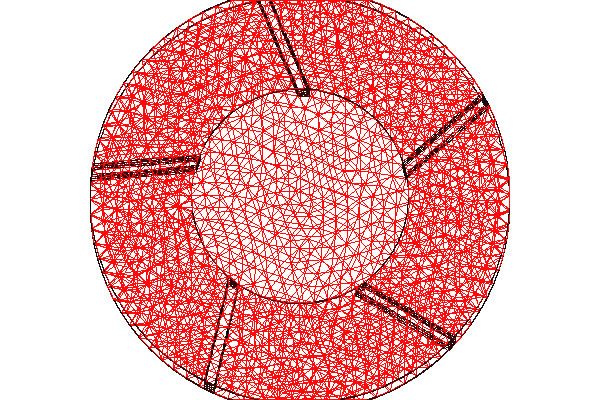
\includegraphics[scale=0.15037593985]{./Figures/Image_8.png}
 &  \\ Case 3. Pressure on Cut Plane &  \\
\end{tabular}
\caption{\label{fig:case 3}
Case 3}
\end{center}
\end{figure}
\vfill
\newpage
\clearpage
\section{Conclusions}


Successful CFD modeling of heatsink.
\\
\end{document}
